% =====================================================================
%  Who Else Asked? Reuse and Leakage in Access-Aware KV-Cache Sharing
%  for Multi-Tenant Retrieval-Augmented Generation
%
%  ACL Rolling Review submission draft (official ACL style, review mode).
%  * All numbers come from numbers.tex / tables/*.tex, generated by
%    scripts/make_paper_assets.py from the committed result files.
%  * \tbd marks measurements that require the pending A100 runs
%    (scripts/sol_array.sbatch); re-running make_paper_assets.py after
%    those runs fills tables/live_v2.tex automatically.
%  * Citations marked VERIFY / TODO in custom.bib are placeholders.
% =====================================================================
\documentclass[11pt]{article}

% "review" = anonymous, line numbers; "final" = camera-ready; "preprint" = arXiv
\usepackage[review]{acl}

\usepackage{times}
\usepackage{latexsym}
\usepackage[T1]{fontenc}
\usepackage[utf8]{inputenc}
\usepackage{microtype}
\usepackage{inconsolata}
\usepackage{graphicx}
\usepackage{booktabs}
\usepackage{amsmath}
\usepackage{amssymb}
\usepackage{amsthm}
\usepackage{xcolor}
\usepackage{xspace}
\usepackage{algorithm}
\usepackage{algpseudocode}
\usepackage{tikz}
\usetikzlibrary{arrows.meta,positioning,fit,calc,decorations.pathreplacing}

% generated by scripts/make_paper_assets.py -- do not edit by hand
\newcommand{\numaclkvRetainHQ}{91}
\newcommand{\numaclkvRetainMQ}{91}
\newcommand{\numaclkvVsPerUserHQ}{5.0}
\newcommand{\numaclkvVsPerUserMQ}{9.2}
\newcommand{\numalignOffACLKV}{4.78}
\newcommand{\numalignOffACLScope}{4.32}
\newcommand{\numalignOnACLKV}{5.68}
\newcommand{\numalignOnACLScope}{5.17}
\newcommand{\numanonLtFiveACLKV}{32.3}
\newcommand{\numbypassGlobal}{60,876}
\newcommand{\numdevTestGap}{0.10}
\newcommand{\numdistinctHQ}{1,605}
\newcommand{\numdistinctMQ}{1,046}
\newcommand{\numdocsForty}{1.9}
\newcommand{\numdocsSeenHQ}{63}
\newcommand{\numdocsTen}{10.5}
\newcommand{\numdocsTwenty}{4.6}
\newcommand{\numexactACLKV}{8.3}
\newcommand{\numexactACLScope}{8.2}
\newcommand{\numexactACLScopeTree}{9.1}
\newcommand{\numexactBinary}{5.7}
\newcommand{\numexactDivergence}{4.9}
\newcommand{\numexactGlobal}{8.3}
\newcommand{\numexactGlobalTree}{9.2}
\newcommand{\numexactNoCache}{0.0}
\newcommand{\numexactPerUser}{1.4}
\newcommand{\numexactSetExact}{54}
\newcommand{\numexactSetHQ}{11}
\newcommand{\numfidMAE}{0.055}
\newcommand{\numfidMax}{0.55}
\newcommand{\numfidN}{192}
\newcommand{\numfidR}{0.99997}
\newcommand{\numgeomEight}{7.1}
\newcommand{\numgeomSeven}{10.5}
\newcommand{\numgeomThirtyTwo}{5.9}
\newcommand{\numgoldMidLCR}{19.7}
\newcommand{\numgoldMidRetrieval}{31.4}
\newcommand{\numgoldMidTree}{32.6}
\newcommand{\numhqACLKV}{5.67}
\newcommand{\numhqACLScope}{5.20}
\newcommand{\numhqACLScopeTree}{6.25}
\newcommand{\numhqBinary}{4.95}
\newcommand{\numhqDivergence}{4.67}
\newcommand{\numhqFourACLKV}{6.69}
\newcommand{\numhqFourACLScope}{5.84}
\newcommand{\numhqFourACLScopeTree}{7.93}
\newcommand{\numhqFourBinary}{5.31}
\newcommand{\numhqFourDivergence}{4.73}
\newcommand{\numhqFourGlobal}{5.84}
\newcommand{\numhqFourGlobalTree}{7.94}
\newcommand{\numhqFourNoCache}{0.00}
\newcommand{\numhqFourPerUser}{2.02}
\newcommand{\numhqGlobal}{5.20}
\newcommand{\numhqGlobalTree}{6.25}
\newcommand{\numhqNoCache}{0.00}
\newcommand{\numhqPerUser}{1.13}
\newcommand{\numkanonRetainSixteen}{69}
\newcommand{\numkvEightACLKV}{8.0}
\newcommand{\numkvEightACLScope}{6.8}
\newcommand{\numkvEightACLScopeTree}{10.5}
\newcommand{\numkvEightPerUser}{3.3}
\newcommand{\numkvFourACLKV}{6.6}
\newcommand{\numkvFourACLScope}{5.7}
\newcommand{\numkvFourACLScopeTree}{7.7}
\newcommand{\numkvFourPerUser}{2.0}
\newcommand{\numkvOneACLKV}{5.1}
\newcommand{\numkvOneACLScope}{4.9}
\newcommand{\numkvOneACLScopeTree}{5.4}
\newcommand{\numkvOnePerUser}{0.6}
\newcommand{\numkvSixteenACLKV}{9.9}
\newcommand{\numkvSixteenACLScope}{8.5}
\newcommand{\numkvSixteenACLScopeTree}{14.3}
\newcommand{\numkvSixteenPerUser}{4.5}
\newcommand{\numkvTwoACLKV}{5.7}
\newcommand{\numkvTwoACLScope}{5.2}
\newcommand{\numkvTwoACLScopeTree}{6.2}
\newcommand{\numkvTwoPerUser}{1.1}
\newcommand{\numliveBoneCached}{3.6}
\newcommand{\numliveBoneRPS}{8.5}
\newcommand{\numliveBoneTTFT}{1461}
\newcommand{\numliveBsixCached}{41.2}
\newcommand{\numliveBsixRPS}{13.7}
\newcommand{\numliveBsixTTFT}{743}
\newcommand{\numliveBthreeTTFT}{1352}
\newcommand{\nummeanPromptHQ}{1393}
\newcommand{\nummeanPromptMQ}{2643}
\newcommand{\numminAnonACLKV}{2}
\newcommand{\nummixDefault}{6.2}
\newcommand{\nummixOpen}{6.0}
\newcommand{\nummixRestrictive}{7.4}
\newcommand{\nummqACLKV}{3.50}
\newcommand{\nummqACLScope}{2.84}
\newcommand{\nummqACLScopeTree}{3.84}
\newcommand{\nummqBinary}{2.69}
\newcommand{\nummqDivergence}{2.47}
\newcommand{\nummqGlobal}{2.84}
\newcommand{\nummqGlobalTree}{3.84}
\newcommand{\nummqNoCache}{0.00}
\newcommand{\nummqPerUser}{0.38}
\newcommand{\numnProbes}{1,362}
\newcommand{\numnoiseFloorMax}{6}
\newcommand{\numordBsix}{4.32}
\newcommand{\numordEdge}{4.89}
\newcommand{\numordLCR}{4.32}
\newcommand{\numordPrivTreeK}{5.17}
\newcommand{\numordRetrieval}{4.59}
\newcommand{\numordTree}{5.69}
\newcommand{\numordTreeK}{5.18}
\newcommand{\numoverstate}{6.6}
\newcommand{\numpadFrac}{5.5}
\newcommand{\numpassageTokensHQ}{128}
\newcommand{\numpassageTokensMQ}{114}
\newcommand{\numpassagesHQ}{66,635}
\newcommand{\numpassagesMQ}{21,100}
\newcommand{\numpicAclHQ}{7.47}
\newcommand{\numpicAclMQ}{8.12}
\newcommand{\numpicGlobalUnauthMQ}{25}
\newcommand{\numpicScopeCost}{0.01}
\newcommand{\numpinACLKV}{32.8}
\newcommand{\numpinACLScope}{32.5}
\newcommand{\numpinACLScopeTree}{33.2}
\newcommand{\numpinBinary}{32.3}
\newcommand{\numpinDivergence}{8.5}
\newcommand{\numpinGlobal}{32.5}
\newcommand{\numpinGlobalTree}{33.2}
\newcommand{\numpinNoCache}{0.0}
\newcommand{\numpinPerUser}{5.7}
\newcommand{\numprefixTreeHQ}{6.18}
\newcommand{\numprefixTreeMQ}{4.00}
\newcommand{\numprivTailCostExact}{0.04}
\newcommand{\numprivTailCostHQ}{0.00}
\newcommand{\numprobeBypassBthree}{137}
\newcommand{\numprobeBypassUB}{19}
\newcommand{\numprobeColdUB}{128}
\newcommand{\numpublicEvidenceHQ}{78}
\newcommand{\numqueryRevealedVone}{99.6}
\newcommand{\numquestionsHQ}{7,377}
\newcommand{\numquestionsMQ}{2,417}
\newcommand{\numrecallHQ}{0.72}
\newcommand{\numrecallMQ}{0.52}
\newcommand{\numrepeatGapHQ}{284}
\newcommand{\numrepeatGapMQ}{229}
\newcommand{\numretBmTwoFiveACLKV}{5.67}
\newcommand{\numretBmTwoFiveACLScopeTree}{6.25}
\newcommand{\numretBmTwoFivePerUser}{1.13}
\newcommand{\numretDenseACLKV}{4.95}
\newcommand{\numretDenseACLScopeTree}{5.43}
\newcommand{\numretDensePerUser}{0.94}
\newcommand{\numretHybridACLKV}{5.39}
\newcommand{\numretHybridACLScopeTree}{5.93}
\newcommand{\numretHybridPerUser}{1.05}
\newcommand{\numrevealACLKV}{44.3}
\newcommand{\numrevealKten}{9.2}
\newcommand{\numsingledACLScope}{91.5}
\newcommand{\numsingledACLScopeMQ}{89.6}
\newcommand{\numsingledBinary}{49.2}
\newcommand{\numsingledKtwo}{2.4}
\newcommand{\numstabLastMQ}{40.4}
\newcommand{\numstabTenHQ}{14.0}
\newcommand{\numstabTenHQShort}{2.2}
\newcommand{\numstabTopHQ}{27.4}
\newcommand{\numstabTopHQShort}{5.2}
\newcommand{\numstabTopMQ}{52.1}
\newcommand{\numtailCostMax}{0.00}
\newcommand{\numtopEdgeTree}{76.6}
\newcommand{\numtreeGainExact}{0.90}
\newcommand{\numtreeGainHQ}{1.05}
\newcommand{\numtreeGainNoiseFifteen}{1.27}
\newcommand{\numtreeGainNoiseFifty}{0.66}
\newcommand{\numtreeWinMax}{6.22}
\newcommand{\numtreeWinMin}{6.16}
\newcommand{\numttftRtwoFour}{0.984}
\newcommand{\numttftRtwoSixteen}{0.998}
\newcommand{\numttftSlopeFour}{0.147}
\newcommand{\numttftSlopeSixteen}{0.92}
\newcommand{\numusersACLScopeFiveHundred}{5.33}
\newcommand{\numusersACLScopeHundred}{5.17}
\newcommand{\numusersACLScopeTwenty}{5.23}
\newcommand{\numusersPerUserFiveHundred}{0.30}
\newcommand{\numusersPerUserHundred}{1.14}
\newcommand{\numusersPerUserTwenty}{3.58}
\newcommand{\numusersRatioFiveHundred}{17.8}
\newcommand{\numusersRatioHundred}{4.5}
\newcommand{\numusersRatioTwenty}{1.5}
\newcommand{\numvOneCIhigh}{+0.074}
\newcommand{\numvOneCIlow}{-0.025}


\newcommand{\sysname}{\textsc{AclKV}\xspace}
\newcommand{\tbd}{\textcolor{red}{\textbf{TBD}}}
\newcommand{\aud}{\mathrm{Aud}}
\newcommand{\acl}{\mathrm{ACL}}
\newtheorem{proposition}{Proposition}
\newtheorem{definition}{Definition}

\title{Who Else Asked? Reuse and Leakage in Access-Aware KV-Cache Sharing\\for Multi-Tenant Retrieval-Augmented Generation}

% Author block is hidden in review mode; fill in for the camera-ready version.
\author{Anonymous ACL submission}

\begin{document}
\maketitle

% ---------------------------------------------------------------------------
\begin{abstract}
Retrieval-augmented generation (RAG) services prefill the same retrieved passages for many users, and prefix caching could reuse that computation. Because a shared cache leaks through response timing, serving engines isolate caches per user and forfeit reuse even among users who are entitled to read the same documents. We study \emph{access-aware} KV-cache sharing, in which cache scopes are derived from the access-control lists (ACLs) of retrieved documents. We prove that ACL-derived scopes cost no reuse relative to unrestricted sharing, but we show that they open an insider channel that per-user isolation does not have: a co-authorized colleague who re-asks a guessed question learns from cache hits whether a colleague asked it, singling out an individual in \numsingledACLScope\% of probes and recovering the question text itself in \numqueryRevealedVone\% when queries inherit the scope of their evidence. We present \sysname, which keeps queries in a private scope and promotes an evidence prefix to a shared scope only after $k$ distinct authorized users have requested it. On retrieval-driven multi-tenant workloads built from HotpotQA and MuSiQue, \sysname eliminates singling-out while retaining \numaclkvRetainHQ\% of the reuse of unrestricted cache-aware sharing (\numaclkvVsPerUserHQ--\numaclkvVsPerUserMQ$\times$ that of per-user isolation); its advantage grows with the number of tenants and with shared context. A simulator validated against \numfidN{} live vLLM runs (mean error \numfidMAE{} points) also shows that workloads which inject popular documents synthetically overstate reuse by \numoverstate$\times$.
\end{abstract}

% ---------------------------------------------------------------------------
\section{Introduction}
\label{sec:intro}

Retrieval-augmented generation \citep{lewis2020rag} conditions a language model on passages retrieved for each query. In enterprise deployments the retrieved evidence dominates the prompt: in our workloads a request carries \nummeanPromptHQ{} (HotpotQA) to \nummeanPromptMQ{} (MuSiQue) prompt tokens, almost all of them evidence, and every token must be prefilled before the first output token appears. Serving engines such as vLLM \citep{kwon2023vllm} and SGLang \citep{zheng2024sglang} avoid recomputing a prompt prefix that an earlier request already processed by caching its key--value (KV) states in fixed-size blocks and reusing them on an exact prefix match \citep{vllm2026apc}.

Sharing those blocks across users is, however, a timing side channel: a cache hit shortens time-to-first-token (TTFT), so a user can test whether someone else recently sent a given prefix and, token by token, reconstruct other users' prompts \citep{wu2025promptpeek,zheng2024inputsnatch,song2024earlybird}. Audits have found prompt caches shared across customers of commercial APIs \citep{gu2025audit}. The standard mitigation is to isolate the cache per user or per request with a secret salt mixed into the first block hash \citep{vllm2026security,addagada2026kvgov}. Isolation is safe, but it also prevents two colleagues who read the \emph{same} company handbook from sharing a single byte of KV state.

Enterprise RAG systems already know who may read each document: retrieval is filtered by document ACLs. This suggests deriving cache scopes from ACLs instead of from user identities, so that users who are jointly authorized for an evidence prefix share it while everyone else is isolated. Engines are beginning to support the required mechanism, several salt barriers inside one request \citep{vllm2025rfc,vllm2026saltregions}. This paper asks two questions. \emph{How much reuse does access-aware sharing recover under realistic multi-tenant RAG traffic?} And \emph{is it actually safe?}

Our answers are mixed, and we believe that this is the useful result:

\begin{itemize}
\item \textbf{ACL scopes are free.} For traffic that passed the authorization filter, ACL-derived scopes produce exactly the cache hits of unrestricted sharing (Proposition~\ref{prop:free}); they cost nothing and fully block clients that reach the engine without server-issued scope identifiers.
\item \textbf{ACL scopes leak to insiders.} A co-authorized colleague can still learn about other users' requests. If the question inherits the scope of its evidence, as in a natural design (including our own first prototype), the colleague recovers the question text in \numqueryRevealedVone\% of probes. Even with private questions, the \emph{sequence of retrieved passages} fingerprints the question: \numsingledACLScope\% of probes single out exactly one colleague who asked it. Per-user isolation has neither channel.
\item \textbf{\sysname closes the channel cheaply.} Keeping the question in a per-user scope costs at most \numprivTailCostExact{} points of reuse, and \emph{$k$-anonymous promotion}, which shares an evidence prefix only after $k$ distinct authorized users requested it, reduces singling-out to 0\% while retaining \numaclkvRetainHQ\% of the reuse of unrestricted cache-aware sharing.
\item \textbf{Realistic gains are modest at small budgets and grow with scale.} When overlap comes from a real retriever rather than from injected documents, access-aware sharing caches \numhqACLKV\% of prompt tokens at a 2\,GiB KV budget versus \numhqPerUser\% for per-user isolation; the gap grows to \numusersRatioFiveHundred$\times$ with 500 tenants, to \numkvSixteenACLScopeTree\% reuse at 16\,GiB, and to \numpinACLKV\% when tenants share pinned context.
\end{itemize}

\noindent We release the middleware, a 60-line vLLM plugin, a prefix-cache simulator validated against \numfidN{} live A100 runs, and the retrieval-driven multi-tenant workloads.\footnote{Code and data: \url{https://anonymous.4open.science/r/aclkv} (anonymized for review).}

% ---------------------------------------------------------------------------
\section{Background and Threat Model}
\label{sec:background}

\paragraph{Prefix caching.} vLLM stores KV states in blocks of $B$ tokens ($B{=}16$). The hash of block $j$ chains over the previous block, $h_j = H(h_{j-1}, \mathbf{t}_j, x_j)$, where $\mathbf{t}_j$ are the block's token ids and $x_j$ optional extra keys. A request reuses its longest prefix of blocks whose hashes are cached; only full blocks are cached, and at least one token is always recomputed. A per-request \texttt{cache\_salt} is mixed into $x_1$ only, so it isolates the entire request through the hash chain \citep{vllm2026security}. A pending proposal generalises this to \emph{salt regions}, i.e.\ $(\text{offset}, \text{salt})$ transitions within a request \citep{vllm2025rfc,vllm2026saltregions}.

\paragraph{Threat model.} The RAG middleware (retriever, authorization filter, prompt builder) and the serving engine are trusted; scope identifiers are derived with a secret server key. We consider two adversaries. A \emph{bypass} client can submit raw token sequences to the engine (e.g., through a misconfigured internal endpoint) but cannot mint scope identifiers. An \emph{insider} is an authenticated employee who uses the RAG front end as intended: they may ask any question, observe TTFT, and read every document their ACLs allow. We give the insider an upper-bound oracle: they learn exactly which blocks hit (in practice TTFT reveals this; Section~\ref{sec:live}) and their guessed question reproduces the victim's evidence. The insider's goal is to learn \emph{whether, and which,} colleagues asked a question. Compromise of the middleware or key, leakage through generated answers, and physical side channels are out of scope.

% ---------------------------------------------------------------------------
\section{Problem Formulation}
\label{sec:problem}

Let $U$ be users and $G$ groups with membership $M\subseteq U\times G$. Every passage $d$ carries an ACL $a(d)$, a conjunction of atoms \texttt{public}, \texttt{group:}$g$, or \texttt{user:}$u$, with audience $\aud(a)\subseteq U$. A request $r=(u, q, D)$ consists of a user, a question, and retrieved passages $D=(d_1,\dots,d_n)$ that passed the authorization filter, i.e.\ $u\in\aud(a(d_i))$ for all $i$. The prompt is $\pi(r) = \sigma \,\Vert\, d_{o(1)} \Vert \cdots \Vert\, d_{o(n)} \,\Vert\, \tau(q)$ for a system preamble $\sigma$, an evidence order $o$, and a question template $\tau$.

Because KV states depend on all preceding tokens, the state of an evidence prefix $P_k=\sigma\,d_{o(1)}\cdots d_{o(k)}$ inherits the restrictions of every passage in it. Its \emph{effective ACL} is
\begin{align}
\acl(P_k) &= \textstyle\bigwedge_{i\le k} a(d_{o(i)}),\\
\aud(\acl(P_k)) &= \textstyle\bigcap_{i\le k}\aud(a(d_{o(i)})).
\end{align}
A \emph{scope assignment} $\zeta$ maps each prompt segment to a scope identifier that is mixed into the hash of the block where the scope begins; later blocks inherit it through the chain.

\begin{definition}[Requirements]
A scope assignment must satisfy, for every request by $u$ that hits a block computed by another request:
\textbf{(S1) authorization}: $u\in\aud(\acl(P))$ for the evidence prefix $P$ that the block ends;
\textbf{(S2) query privacy}: the block contains no question tokens of another user;
\textbf{(S3) $k$-anonymity}: at least $k{-}1$ users other than $u$ have requested the same evidence prefix.
Moreover, \textbf{(S0) bypass resistance}: a request without server-issued scope identifiers hits no scoped block.
\end{definition}

\noindent The objective is to maximize the number of reused prompt tokens under a fixed KV-cache budget subject to S0--S3. Per-user isolation satisfies all requirements with almost no reuse; unrestricted sharing violates all of them.

\begin{proposition}[ACL scopes are reuse-free]
\label{prop:free}
Let $\zeta_{\acl}(P)=\mathrm{HMAC}_K(\mathrm{canon}(\acl(P)))$ and suppose a passage's ACL is a function of its content. For every trace of requests that passed the authorization filter, the evidence blocks hit under $\zeta_{\acl}$ are exactly those hit under unrestricted sharing, and S0 and S1 hold.
\end{proposition}
\begin{proof}[Proof sketch]
If two prompts agree on their first $j$ blocks, they contain the same passages in the same order up to block $j$, so their effective ACLs, and hence their scope identifiers, agree on those blocks; scoping therefore never separates two prompts that unrestricted sharing would let share. For S1, a hit by $u$ on a block ending prefix $P$ means $u$'s own prompt contains $P$, every passage of which passed $u$'s filter, so $u\in\aud(\acl(P))$. For S0, unscoped hashes differ from scoped ones on the first block of every scope.
\end{proof}

\noindent Proposition~\ref{prop:free} has a sobering corollary: for honest traffic, the authorization filter alone already guarantees S1, and \emph{all} of the privacy cost of access-aware sharing comes from S2 and S3, which ACL scopes do not provide. Our experiments confirm both halves (Sections~\ref{sec:main} and~\ref{sec:privacy}).

% ---------------------------------------------------------------------------
\section{\sysname}
\label{sec:method}

\begin{figure*}[t]
\centering
\resizebox{\textwidth}{!}{%
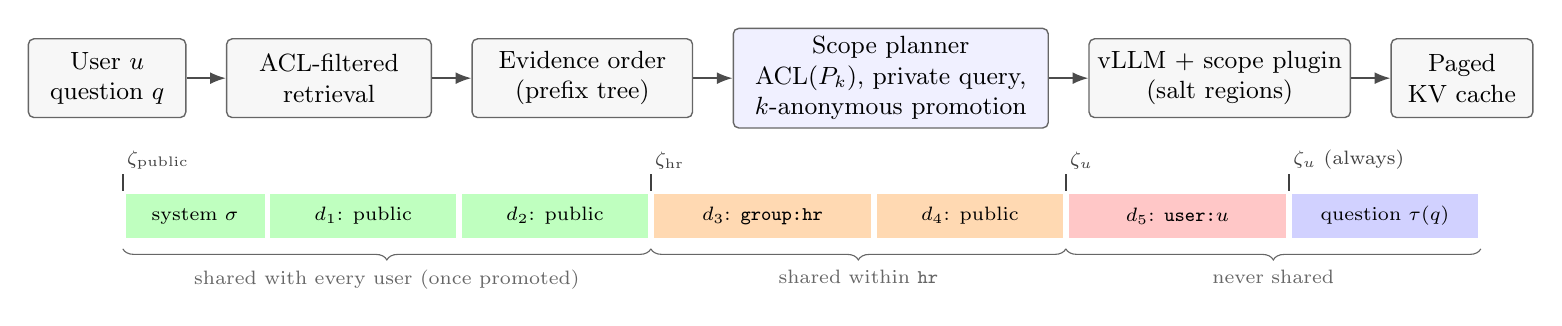
\begin{tikzpicture}[
  font=\small,
  box/.style={rounded corners=2pt, draw=black!60, line width=.5pt, align=center, minimum height=10mm, inner sep=3pt, fill=black!3},
  arr/.style={-{Latex[length=2mm]}, line width=.6pt, draw=black!70},
  seg/.style={draw=white, line width=1pt, minimum height=6mm, inner sep=1pt, font=\scriptsize, text=black}
]
\node[box, minimum width=20mm] (q) {User $u$\\question $q$};
\node[box, right=5mm of q, minimum width=26mm] (ret) {ACL-filtered\\retrieval};
\node[box, right=5mm of ret, minimum width=28mm] (ord) {Evidence order\\(prefix tree)};
\node[box, right=5mm of ord, minimum width=40mm, fill=blue!6] (scope) {Scope planner\\$\acl(P_k)$, private query,\\$k$-anonymous promotion};
\node[box, right=5mm of scope, minimum width=30mm] (eng) {vLLM + scope plugin\\(salt regions)};
\node[box, right=5mm of eng, minimum width=18mm] (kv) {Paged\\KV cache};
\draw[arr] (q) -- (ret); \draw[arr] (ret) -- (ord); \draw[arr] (ord) -- (scope); \draw[arr] (scope) -- (eng); \draw[arr] (eng) -- (kv);
% prompt layout strip
\begin{scope}[shift={(0.2,-1.75)}]
\node[seg, fill=green!25, minimum width=18mm, anchor=west] (s0) at (0,0) {system $\sigma$};
\node[seg, fill=green!25, minimum width=24mm, right=0mm of s0] (s1) {$d_1$: public};
\node[seg, fill=green!25, minimum width=24mm, right=0mm of s1] (s2) {$d_2$: public};
\node[seg, fill=orange!30, minimum width=28mm, right=0mm of s2] (s3) {$d_3$: \texttt{group:hr}};
\node[seg, fill=orange!30, minimum width=24mm, right=0mm of s3] (s4) {$d_4$: public};
\node[seg, fill=red!22, minimum width=28mm, right=0mm of s4] (s5) {$d_5$: \texttt{user:}$u$};
\node[seg, fill=blue!18, minimum width=24mm, right=0mm of s5] (s6) {question $\tau(q)$};
\foreach \n/\lab in {s0/{$\zeta_{\text{public}}$}, s3/{$\zeta_{\text{hr}}$}, s5/{$\zeta_{u}$}, s6/{$\zeta_{u}$ (always)}} {
  \draw[line width=.9pt, black!75] (\n.north west) -- ++(0,0.22) node[above right, inner sep=1pt, font=\scriptsize] {\lab};
}
\draw[decorate, decoration={brace, mirror, amplitude=4pt}, black!60] ([yshift=-1mm]s0.south west) -- ([yshift=-1mm]s2.south east) node[midway, below=4pt, font=\scriptsize] {shared with every user (once promoted)};
\draw[decorate, decoration={brace, mirror, amplitude=4pt}, black!60] ([yshift=-1mm]s3.south west) -- ([yshift=-1mm]s4.south east) node[midway, below=4pt, font=\scriptsize] {shared within \texttt{hr}};
\draw[decorate, decoration={brace, mirror, amplitude=4pt}, black!60] ([yshift=-1mm]s5.south west) -- ([yshift=-1mm]s6.south east) node[midway, below=4pt, font=\scriptsize] {never shared};
\end{scope}
\end{tikzpicture}}
\caption{\sysname. Top: the serving path; the only engine change is a block-hash extra key per scope barrier. Bottom: a prompt with its scope barriers ($\zeta$). Each barrier is placed where the effective ACL of the evidence prefix narrows; later blocks inherit it through the hash chain, so the public passage $d_4$ placed after $d_3$ is shared only within \texttt{hr}. The question is always in the user's private scope, and a shared barrier takes effect only after $k$ distinct authorized users requested that prefix.}
\label{fig:overview}
\end{figure*}

\sysname is middleware between retrieval and the serving engine (Figure~\ref{fig:overview}).

\paragraph{ACL-derived scope barriers.} For the ordered evidence, the planner computes $\acl(P_k)$ incrementally and emits a barrier $(\text{offset}, \zeta)$ wherever it changes, with $\zeta=\mathrm{HMAC}_K(\mathrm{canon}(\acl(P_k)))$ truncated to 64 bits. Identifiers are server-derived and fixed-size, the number of barriers is bounded, and the encoded list stays far below the engine's salt-length limit, which avoids a recently disclosed denial-of-service vector \citep{vllm2026dos}. We transport the barriers in vLLM's existing \texttt{cache\_salt} field and add a 60-line general plugin that keys each scope into the block containing its offset; malformed salts fail closed to request-level isolation, and ordinary salts keep their stock semantics. The same barriers map one-to-one onto the proposed native \texttt{salt\_regions} API \citep{vllm2026saltregions}. The middleware sends token ids rather than text, so barrier offsets are exact, and pads each segment to a block boundary so that a passage's blocks never depend on the length of its predecessor.

\paragraph{Private query scope.} The question template $\tau(q)$, and therefore every generated token, is always placed in the requester's own scope $\mathrm{HMAC}_K(\texttt{user:}u)$. A user still reuses their own repeated questions, but no other user can hit them (S2).

\paragraph{$k$-anonymous promotion.} Algorithm~\ref{alg:promote} enforces S3. The middleware counts, for each pair (effective ACL, evidence prefix), the distinct users who requested it. A segment uses its shared ACL scope only if the requester would be at least the $k$-th distinct requester and the prefix's audience has at least $k$ members; otherwise that segment, and every later one, uses the requester's private scope. A cross-user hit therefore reveals only that at least $k{-}1$ other users asked for the same evidence \citep{sweeney2002kanon}. The counter is a bounded LRU map; an evicted prefix must be re-promoted, which fails closed.

\begin{algorithm}[t]
\caption{Scope plan with $k$-anonymous promotion}
\label{alg:promote}
\small
\begin{algorithmic}[1]
\Require user $u$; segments $s_0{=}\sigma,s_1,\dots,s_{n+1}{=}\tau(q)$
\Require counter $C$; threshold $k$
\State $A\gets\texttt{public}$;\; $\textit{private}\gets\textbf{false}$
\For{$i=0$ \textbf{to} $n$}
  \State \textbf{if} $i\ge1$ \textbf{then} $A\gets A\wedge a(s_i)$
  \State $key\gets(\mathrm{canon}(A), \mathrm{digest}(s_1..s_i))$
  \If{$\neg\textit{private}$ \textbf{and} ($|\aud(A)|<k$ \textbf{or} $|C[key]\cup\{u\}|<k$)}
     \State $\textit{private}\gets\textbf{true}$
  \EndIf
  \State $\zeta_i\gets$ \textbf{if} $\textit{private}$ \textbf{then} $\mathrm{HMAC}_K(\texttt{user:}u)$ \textbf{else} $\mathrm{HMAC}_K(\mathrm{canon}(A))$
  \State $C[key]\gets C[key]\cup\{u\}$
\EndFor
\State $\zeta_{n+1}\gets\mathrm{HMAC}_K(\texttt{user:}u)$ \Comment{private query}
\State \Return barriers where $\zeta_i\ne\zeta_{i-1}$
\end{algorithmic}
\end{algorithm}

\paragraph{Evidence order.} Prefix reuse requires that related requests place shared evidence at the same positions. Following CacheWeaver \citep{tan2026cacheweaver}, \sysname keeps a trie over a sliding window of recently served evidence sequences and greedily places first the passages whose prefix was served most often, followed by the remaining passages in retrieval order. We evaluated two access-aware refinements, a walk that prefers already-promoted prefixes and a layout that places relevant evidence at the edges of the context; neither helped (Section~\ref{sec:ordering}), so \sysname uses the plain tree.

% ---------------------------------------------------------------------------
\section{Experimental Setup}
\label{sec:setup}

\paragraph{Data.} We use the HotpotQA development set \citep{yang2018hotpotqa} (\numquestionsHQ{} questions, \numpassagesHQ{} distinct passages) and MuSiQue-Ans \citep{trivedi2022musique} (\numquestionsMQ{} questions, \numpassagesMQ{} passages). Passages are deduplicated by content; each request retrieves the top 10 (HotpotQA) or 20 (MuSiQue) passages from the \emph{whole} corpus with BM25 \citep{robertson2009bm25}, filtered by the requester's ACLs (gold-passage recall@k is \numrecallHQ{} and \numrecallMQ{}). Conclusions are unchanged with dense (bge-small) or hybrid retrieval, which preserve the ranking of all policies with slightly lower absolute reuse (\sysname: \numretDenseACLKV\% and \numretHybridACLKV\% vs.\ \numretBmTwoFiveACLKV\%; Appendix Table~\ref{tab:retriever}).

\paragraph{Multi-tenant workloads.} We simulate an organization of 100 users in 10 departments nested in 3 divisions, plus 6 cross-functional groups with overlapping membership. Questions are clustered into 40 balanced topics (LSA $k$-means with capacity-constrained assignment); each topic is owned by a department. A passage is public with probability $0.5$; otherwise it is restricted to its owning department, that department's division, or a cross-functional group ($0.3$), or is private to one department member ($0.2$). Users ask about their own department's topics with probability $0.8$, and questions within a topic follow a Zipf distribution, so popular questions recur. To model paraphrases, 30\% of a question's content terms are dropped \emph{for retrieval only}; the prompt keeps the original question. Each workload has 5{,}000 requests with \numdistinctHQ{} (HotpotQA) and \numdistinctMQ{} (MuSiQue) distinct questions; \numexactSetHQ\% of requests repeat an evidence set exactly, yet \numdocsSeenHQ\% of their passages were retrieved before. Crucially, cross-request overlap is produced by the retriever, never injected. Variants change the number of tenants, ACL mix, paraphrase noise, and passages per request, and add 4 always-included public passages (\emph{pinned}, e.g.\ a handbook). Appendix~\ref{app:workloads} gives details.

\paragraph{Policies.} \emph{No caching}; \emph{per-user salt} (vLLM's mitigation and KVGov's per-principal salt; \citealp{vllm2026security,addagada2026kvgov}); \emph{divergence salt} (shared system preamble, per-user afterwards; KVGov's divergence variant); \emph{public/private split} (one boundary at the first non-public passage, the binary model of SafeKV with oracle labels; \citealp{chu2025safekv}); \emph{ACL scopes} with retrieval order and with tree order; \sysname ($k{=}3$); and two insecure upper bounds, \emph{global} sharing with retrieval and with tree order (the latter is CacheWeaver as published). All secure policies use a private question scope unless stated otherwise.

\paragraph{Metrics.} Efficiency: cached prompt tokens (\%), recomputed tokens per request, evictions. Privacy: after 10\% of requests a randomly chosen co-authorized insider re-issues the victim's question through the middleware (\numnProbes{} probes per policy on HotpotQA). A hit is \emph{informative} if the block was computed only by other users; its \emph{anonymity set} is the set of distinct other users who had requested that exact evidence prefix (or that exact question) at any earlier point. Using all history enlarges the anonymity sets of the baselines and is therefore conservative for our defence. We report the fraction of probes that reveal anything, that \emph{single out} one user (anonymity set of size one), that have an anonymity set smaller than 5, and that hit the question text. Bypass probes replay a victim's tokens without scope identifiers. Quality: EM and F1 against gold answers and aliases, with question-clustered bootstrap confidence intervals.

\paragraph{Platform and protocol.} Large sweeps use a trace-driven simulator that mirrors vLLM~0.29's block manager (chained block hashes, the $n{-}1$ hit cap, LRU free queue, reverse-order release, touch-on-hit) with a closed loop of 16 concurrent requests, 48 output tokens, and Qwen2.5-7B-Instruct's KV geometry \citep{qwen2025qwen25} (56\,KiB per token; a 2\,GiB budget holds about 37k tokens). Live experiments run vLLM~0.29 on one NVIDIA A100-80GB with an explicit KV budget. All design decisions were made on HotpotQA seed~0; HotpotQA seeds 1--2 and all MuSiQue seeds are held out, and seed-0 values differ from held-out means by at most \numdevTestGap{} points.

% ---------------------------------------------------------------------------
\section{Results}
\label{sec:results}

\subsection{Simulator fidelity and the latency model}
\label{sec:fidelity}
We first validate the simulator against a pilot study of \numfidN{} live A100 runs (Appendix~\ref{app:pilot}): for every run we rebuilt the prompts locally (identical evidence order in all requests) and replayed them with the live completion lengths. Simulated and live cached-token fractions agree with a mean absolute error of \numfidMAE{} points (maximum \numfidMax, $r=\numfidR$; Appendix Figure~\ref{fig:fidelity}). Live mean TTFT is a linear function of recomputed prompt tokens per request ($R^2=\numttftRtwoSixteen$ at 16 concurrent requests, \numttftSlopeSixteen{}\,ms per recomputed token; $R^2=\numttftRtwoFour$ at 4). We therefore report cached tokens as the primary efficiency metric for large sweeps and confirm latency on the GPU (Section~\ref{sec:live}).

\subsection{Main comparison}
\label{sec:main}

\begin{table*}[t]
\centering
\small
\begin{tabular}{@{}l l r r r r r@{}}
\toprule
 & & \multicolumn{3}{c}{Cached prompt tokens (\%)} & & Insider \\ \cmidrule(lr){3-5}
Policy & Isolation & HotpotQA & MuSiQue & Pinned & vs.\ per-user & singled-out (\%) \\
\midrule
No caching & full & 0.00$\pm$0.00 & 0.00$\pm$0.00 & 0.0 & -- & 0.0 \\
Per-user salt & per user & 1.13$\pm$0.01 & 0.38$\pm$0.02 & 5.7 & 1.0$\times$ & 0.0 \\
Divergence salt & per user$^{\dagger}$ & 4.67$\pm$0.03 & 2.47$\pm$0.03 & 8.5 & 4.1$\times$ & 0.0 \\
Public/private split & public/user & 4.95$\pm$0.02 & 2.69$\pm$0.02 & 32.3 & 4.4$\times$ & 49.2 \\
ACL scopes & ACL & 5.20$\pm$0.02 & 2.84$\pm$0.05 & 32.5 & 4.6$\times$ & 91.5 \\
ACL scopes + tree order & ACL & 6.25$\pm$0.12 & 3.84$\pm$0.15 & 33.2 & 5.5$\times$ & 93.7 \\
\textbf{\textsc{AclKV} ($k{=}3$)} & ACL + $k$-anon. & \textbf{5.67}$\pm$0.02 & \textbf{3.50}$\pm$0.16 & 32.8 & 5.0$\times$ & 0.0 \\
\midrule
Global sharing & none & 5.20$\pm$0.02 & 2.84$\pm$0.05 & 32.5 & 4.6$\times$ & 91.5 \\
Global + tree order & none & 6.25$\pm$0.12 & 3.84$\pm$0.15 & 33.2 & 5.5$\times$ & 93.7 \\
\bottomrule
\end{tabular}

\caption{Cached prompt tokens at a 2\,GiB KV budget (mean $\pm$ s.d.\ over three workload seeds; \emph{pinned}: one seed), relative reuse versus per-user isolation on HotpotQA, and the fraction of insider probes that single out one colleague. $^\dagger$Shared system preamble. Global sharing is insecure and shown as an upper bound; it also leaks to bypass clients (\numbypassGlobal{} honest blocks hit), unlike every scoped policy (0).}
\label{tab:main}
\end{table*}

Table~\ref{tab:main} summarizes the comparison. Three observations stand out. First, ACL scopes reproduce the reuse of global sharing exactly, as Proposition~\ref{prop:free} predicts (\numhqACLScope\% vs.\ \numhqGlobal\%), and cache-aware tree ordering adds \numtreeGainHQ{} points on top of either. Second, absolute reuse is modest at this budget: the system preamble alone (divergence salt) accounts for \numhqDivergence\% of prompt tokens, and sharing evidence across users adds at most another 1.6 points on HotpotQA and 1.4 on MuSiQue, because a 2\,GiB cache holds only about 27 requests while identical questions recur a median of \numrepeatGapHQ{} (HotpotQA) and \numrepeatGapMQ{} (MuSiQue) requests apart. Third, the picture changes completely when tenants share context: with four pinned public passages, scoped sharing caches \numpinACLScope\% of prompt tokens versus \numpinPerUser\% for per-user and \numpinDivergence\% for divergence salting. \sysname gives up a little reuse for $k$-anonymity (\numhqACLKV\% vs.\ \numhqACLScopeTree\%) and remains \numaclkvVsPerUserHQ$\times$ (HotpotQA) and \numaclkvVsPerUserMQ$\times$ (MuSiQue) more effective than per-user isolation.

\subsection{Insider leakage and the privacy--utility frontier}
\label{sec:privacy}

\begin{table}[t]
\centering
\small
\setlength{\tabcolsep}{3.2pt}
\resizebox{\columnwidth}{!}{\begin{tabular}{@{}l r r r r r r@{}}
\toprule
 & \multicolumn{4}{c}{HotpotQA insider probes (\%)} & MuSiQue & Cached \\ \cmidrule(lr){2-5}
Policy & reveal & single & anon$<$5 & query & single (\%) & (\%) \\
\midrule
Global sharing (insecure) & 100.0 & 91.5 & 99.9 & 99.6 & 90.6 & 5.20 \\
Per-user salt & 0.0 & 0.0 & 0.0 & 0.0 & 0.0 & 1.09 \\
Divergence salt & 0.0 & 0.0 & 0.0 & 0.0 & 0.0 & 4.66 \\
Public/private split & 67.6 & 49.2 & 63.1 & 0.0 & 44.8 & 4.92 \\
ACL scopes, inherited query (v1) & 100.0 & 91.5 & 99.9 & 99.6 & 90.6 & 5.16 \\
ACL scopes & 100.0 & 91.5 & 99.9 & 0.0 & 89.6 & 5.16 \\
ACL scopes + tree order & 100.0 & 93.7 & 99.9 & 0.0 & 95.2 & 6.19 \\
\textsc{AclKV}, $k{=}2$ & 58.4 & 2.4 & 51.3 & 0.0 & 2.3 & 5.79 \\
\textbf{\textsc{AclKV}, $k{=}3$} & 44.3 & \textbf{0.0} & 32.3 & 0.0 & 0.0 & 5.59 \\
\textsc{AclKV}, $k{=}5$ & 27.3 & 0.0 & 3.1 & 0.0 & 0.0 & 5.35 \\
\textsc{AclKV}, $k{=}10$ & 9.2 & 0.0 & 0.0 & 0.0 & 0.0 & 4.98 \\
\bottomrule
\end{tabular}
}
\caption{Insider probes through the middleware (HotpotQA: three seeds; MuSiQue: one seed; 2\,GiB). \emph{reveal}: any informative hit; \emph{single}: anonymity set of one; \emph{query}: hit on the victim's question text. Cached: honest requests in the same trace.}
\label{tab:privacy}
\end{table}

Table~\ref{tab:privacy} shows that access-aware sharing is not leak-free. Under ACL scopes, every insider probe reveals that a colleague recently retrieved the same evidence, and \numsingledACLScope\% (MuSiQue: \numsingledACLScopeMQ\%) single out exactly one colleague; when the question inherits its evidence scope, the insider additionally recovers the question text in \numqueryRevealedVone\% of probes. The public/private split leaks less (\numsingledBinary\%) only because it shares less. Per-user and divergence salting reveal nothing.

$k$-anonymous promotion closes the singling-out channel: with $k{=}3$, no probe singles out a colleague (smallest anonymity set observed: \numminAnonACLKV, as guaranteed), only \numrevealACLKV\% reveal anything, and \numanonLtFiveACLKV\% have an anonymity set below five. Figure~\ref{fig:frontier} traces the frontier: each increase of $k$ trades a few tenths of a point of reuse for a large drop in what an insider learns; at $k{=}10$ only \numrevealKten\% of probes reveal anything, and reuse still exceeds divergence salting.

\begin{figure}[t]
\centering
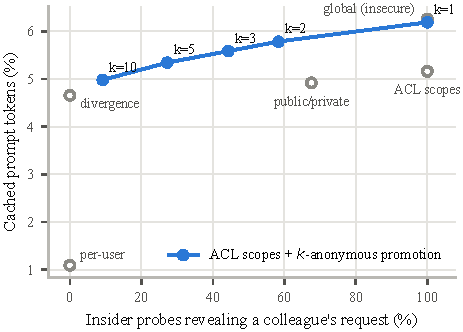
\includegraphics[width=\columnwidth]{figures/frontier.pdf}
\caption{Privacy--utility frontier on HotpotQA (2\,GiB, three seeds). The blue curve varies the promotion threshold $k$ of \sysname; hollow points are baselines.}
\label{fig:frontier}
\end{figure}

\subsection{When does access-aware sharing pay off?}
\label{sec:scaling}

\begin{figure*}[t]
\centering
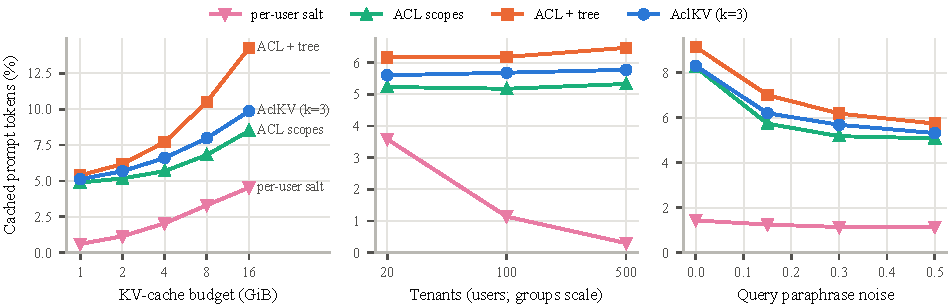
\includegraphics[width=\textwidth]{figures/scaling.pdf}
\caption{Cached prompt tokens on HotpotQA as a function of the KV budget, the number of tenants, and query paraphrase noise. Global sharing with tree order coincides with \emph{ACL + tree} in every setting (Proposition~\ref{prop:free}).}
\label{fig:scaling}
\end{figure*}

Figure~\ref{fig:scaling} varies the deployment. \emph{Tenants:} per-user isolation collapses as the population grows (\numusersPerUserTwenty\% with 20 users, \numusersPerUserFiveHundred\% with 500), whereas ACL scopes are flat (\numusersACLScopeTwenty--\numusersACLScopeFiveHundred\%), so the advantage grows from \numusersRatioTwenty$\times$ to \numusersRatioFiveHundred$\times$. \emph{Budget:} reuse grows with the KV budget for every policy, fastest for tree-ordered sharing (\numkvOneACLScopeTree\% at 1\,GiB to \numkvSixteenACLScopeTree\% at 16\,GiB). The cost of $k$-anonymity grows with the budget too: \sysname retains \numkanonRetainSixteen\% of tree-ordered reuse at 16\,GiB, because a larger cache keeps more question-specific prefixes that never reach $k$ requesters. \emph{Paraphrase noise} reduces reuse for all policies; the gain of tree ordering over retrieval order is largest when evidence sets overlap but are reordered (\numtreeGainNoiseFifteen{} points at 15\% noise versus \numtreeGainExact{} for exact queries and \numtreeGainNoiseFifty{} at 50\%). Appendix Table~\ref{tab:scaling} adds prompt length, model KV geometry, ACL mix, and concurrency: longer prompts and larger per-token KV footprints reduce reuse (Qwen2.5-32B fits 4.6$\times$ fewer tokens per GiB than Qwen2.5-7B), and a more restrictive ACL mix slightly \emph{increases} reuse (\nummixRestrictive\% vs.\ \nummixDefault\% with tree order), plausibly because ACL filtering concentrates each department's retrieval on its own passages.

\subsection{Live serving}
\label{sec:live}

\begin{table}[t]
\centering
\small
\setlength{\tabcolsep}{3pt}
\resizebox{\columnwidth}{!}{\begin{tabular}{@{}l r r r r r@{}}
\toprule
Policy & Cached (\%) & TTFT p50 (ms) & TTFT p95 (ms) & req/s & EM / F1 \\
\midrule
Per-user salt & \tbd & \tbd & \tbd & \tbd & \tbd \\
Divergence salt & \tbd & \tbd & \tbd & \tbd & \tbd \\
ACL scopes & \tbd & \tbd & \tbd & \tbd & \tbd \\
ACL scopes + tree order & \tbd & \tbd & \tbd & \tbd & \tbd \\
\textsc{AclKV} ($k{=}3$) & \tbd & \tbd & \tbd & \tbd & \tbd \\
Global (insecure) & \tbd & \tbd & \tbd & \tbd & \tbd \\
\bottomrule
\end{tabular}
}
\caption{Live vLLM~0.29 on one A100 (Qwen2.5-7B-Instruct, 2\,GiB KV budget, HotpotQA workloads, 2{,}000 requests, 16 concurrent). \tbd: pending runs (\texttt{scripts/sol\_array.sbatch}; Qwen3-8B, Llama-3.1-8B and Qwen2.5-32B and open-loop goodput in Appendix~\ref{app:repro}).}
\label{tab:live}
\end{table}

Table~\ref{tab:live} will report TTFT, throughput, and answer quality measured end-to-end on the GPU for the realistic workloads. \emph{[Pending A100 runs.]} The pilot study already establishes the mechanism on real hardware: with the synthetic-injection workload at 50\% overlap (Appendix~\ref{app:pilot}), cache-aware sharing cut median TTFT from \numliveBoneTTFT\,ms (per-user) to \numliveBsixTTFT\,ms and raised throughput from \numliveBoneRPS{} to \numliveBsixRPS{} requests/s, and the live bypass probe confirmed the timing channel: unscoped replays of a victim's prompt returned in \numprobeBypassUB\,ms versus \numprobeColdUB\,ms cold under global sharing, and hit nothing under ACL scopes (\numprobeBypassBthree\,ms). Given the TTFT model of Section~\ref{sec:fidelity}, we expect the realistic workloads' smaller reuse to translate into proportionally smaller latency gains at 2\,GiB and larger ones at 8\,GiB.

% ---------------------------------------------------------------------------
\section{Analysis and Ablations}
\label{sec:analysis}

\subsection{Evidence order: relevance and reuse are aligned}
\label{sec:ordering}

\begin{table}[t]
\centering
\small
\setlength{\tabcolsep}{3pt}
\resizebox{\columnwidth}{!}{\begin{tabular}{@{}l r r r@{}}
\toprule
Evidence order & Cached (\%) & Gold mid (\%) & Top-1 at edge (\%) \\
\midrule
Retrieval order & 4.59 & 31.4 & 100.0 \\
Broad-to-narrow (v1 B4) & 4.62 & 33.9 & 76.1 \\
Popularity-canonical (v1 B5) & 4.47 & 36.6 & 67.8 \\
+ relevance anchor (v1 B6) & 4.32 & 22.9 & 100.0 \\
LongContextReorder & 4.32 & 19.7 & 100.0 \\
Edge layout & 4.89 & 31.7 & 93.8 \\
Prefix tree (CacheWeaver-style) & 5.69 & 32.6 & 76.6 \\
Prefix tree, $k{=}3$ & 5.18 & 32.6 & 76.6 \\
Privacy-aware tree, $k{=}3$ & 5.17 & 32.6 & 76.6 \\
\bottomrule
\end{tabular}
}
\caption{Evidence ordering under ACL scopes (mean over three HotpotQA seeds and one MuSiQue seed, 2\,GiB). \emph{Gold mid}: answer-bearing passages in positions $3$ to $n{-}2$; \emph{Top-1 at edge}: highest-ranked passage first or last.}
\label{tab:order}
\end{table}

Table~\ref{tab:order} compares orderings. The CacheWeaver-style tree yields the most reuse (\numordTree\% vs.\ \numordRetrieval\% for retrieval order). Two plausible access-aware refinements fail. Our pilot proposed placing the most relevant passages next to the question, motivated by the observation that language models attend most to the edges of a long context \citep{liu2024lost} and that, under synthetic injection, relevant passages were question-specific and shared ones were not. With real retrieval this premise is false: highly ranked passages are the \emph{most} reusable ones (Figure~\ref{fig:stability}; on HotpotQA, \numstabTopHQ\% of rank-1 passages were retrieved by one of the previous 200 requests versus \numstabTenHQ\% of rank-10 passages), so moving them to the end of the prompt shortens shared prefixes (\numordEdge\%; LongContextReorder \citep{langchain2023lcr}: \numordLCR\%). Reuse and relevance therefore both favour the \emph{front} of the context. Second, a privacy-aware walk that prefers already-promoted prefixes is indistinguishable from the plain tree under $k{=}3$ (\numordPrivTreeK\% vs.\ \numordTreeK\%). The tree moves the top-ranked passage away from the first position in a quarter of requests (top-1 at an edge: \numtopEdgeTree\%), which is why we measure answer quality directly (Section~\ref{sec:quality}).

\begin{figure}[t]
\centering
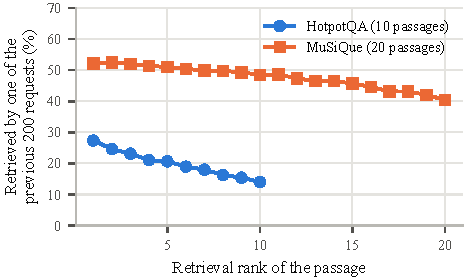
\includegraphics[width=\columnwidth]{figures/stability.pdf}
\caption{Probability that a retrieved passage was retrieved by one of the previous 200 requests, by retrieval rank (three seeds each). Highly relevant passages are the most reusable.}
\label{fig:stability}
\end{figure}

\subsection{Mechanism ablations}
\label{sec:mech}
\emph{Private query scope} costs no measurable reuse on the held-out workloads (below 0.01 points) and \numprivTailCostExact{} points even when questions repeat verbatim (exact-query workload), while removing all question-text leakage (Table~\ref{tab:privacy}). \emph{Block alignment} matters: without padding segments to block boundaries, \sysname caches \numalignOffACLKV\% instead of \numalignOnACLKV\% (padding adds \numpadFrac\% tokens). The tree window is insensitive between 64 and 4{,}096 sequences (\numtreeWinMin--\numtreeWinMax\%).

\subsection{Position-independent caching}
\label{sec:pic}
A natural objection to prefix caching is that the same passage appears in different contexts, which changes the token prefix and prevents reuse. Position-independent caching addresses this directly by caching each passage's KV separately and recomputing a fraction $r$ of tokens to restore cross-passage attention \citep{yao2025cacheblend}. In our simulator (Appendix Table~\ref{tab:pic}), it raises reuse from \numprefixTreeHQ\% to \numpicAclHQ\% on HotpotQA and from \numprefixTreeMQ\% to \numpicAclMQ\% on MuSiQue at $r{=}0.15$. Two findings transfer from Section~\ref{sec:problem}: because a separately encoded passage depends only on itself, its correct scope is its \emph{own} ACL rather than the prefix's, and own-ACL scoping again costs at most \numpicScopeCost{} points relative to unscoped chunk caching; without any scope, chunk caching produced \numpicGlobalUnauthMQ{} unauthorized hits on MuSiQue from honest traffic alone, because passages with different ACLs can share identical leading text. Position-independent reuse is complementary to \sysname but requires engine changes and has its own timing channel \citep{sun2026spliceleak}.

\subsection{Answer quality}
\label{sec:quality}

\begin{table}[t]
\centering
\small
\setlength{\tabcolsep}{3pt}
\resizebox{\columnwidth}{!}{\begin{tabular}{@{}l r r r r@{}}
\toprule
Overlap & ACL-scope F1 & $\Delta$F1 v1-B5 & $\Delta$F1 v1-B6 [95\% CI] & $p$ \\
\midrule
0.00 & 0.685 & -0.004 & +0.017 [-0.023, +0.056] & 0.42 \\
0.25 & 0.681 & -0.002 & +0.023 [-0.023, +0.074] & 0.34 \\
0.50 & 0.649 & -0.002 & +0.029 [-0.015, +0.074] & 0.20 \\
0.75 & 0.679 & +0.007 & +0.013 [-0.025, +0.052] & 0.50 \\
\bottomrule
\end{tabular}
}
\caption{Pilot answer quality on the live A100 (HotpotQA, Qwen2.5-7B-Instruct, 400 requests per overlap level). Differences to retrieval order; 95\% question-clustered bootstrap CIs.}
\label{tab:quality}
\end{table}

Cache-aware ordering changes what the model reads first, so it could affect answers. In the pilot (Table~\ref{tab:quality}), neither popularity-canonical ordering nor relevance anchoring changed F1 significantly at any overlap level (all 95\% intervals contain zero; range \numvOneCIlow{} to \numvOneCIhigh). Requests with identical token sequences produced different answers under different salting policies in at most \numnoiseFloorMax{} of 400 cases (numerical differences between cached and recomputed prefill), which bounds the effect of salting itself. The corresponding comparison for tree ordering on the realistic workloads, with an LLM judge in addition to EM/F1, is part of the pending GPU runs (\tbd).

\subsection{Synthetic overlap overstates reuse}
\label{sec:synthetic}
Our pilot followed common practice and created cross-user overlap by injecting popular passages into requests. Under that workload, cache-aware sharing reached \numliveBsixCached\% cached tokens live, \numoverstate$\times$ the \numhqACLScopeTree\% it reaches when overlap comes from retrieval. Injected passages are irrelevant to the question, rank low, and can be moved freely to the front; real shared passages are relevant, rank high, and already sit near the front. We recommend that evaluations of RAG caching derive overlap from a retriever and report it (Section~\ref{sec:setup}).

% ---------------------------------------------------------------------------
\section{Related Work}
\label{sec:related}

\paragraph{Prefix and RAG caching.} PagedAttention \citep{kwon2023vllm} and RadixAttention \citep{zheng2024sglang} reuse exact prompt prefixes; Prompt Cache \citep{gim2024promptcache} reuses modular segments. RAG-specific systems cache knowledge across requests \citep{jin2024ragcache}, precompute or fuse per-passage KV states \citep{yao2025cacheblend,lu2024turborag,sun2024blockattention}, or reorder evidence to create shared prefixes \citep{tan2026cacheweaver}. None of these considers which users may share a cached state; we compose with CacheWeaver-style ordering and show that access control does not change the best order.

\paragraph{KV-cache side channels and defences.} Timing attacks reconstruct prompts from shared prefix caches \citep{wu2025promptpeek,zheng2024inputsnatch,song2024earlybird}, including non-prefix RAG caches \citep{sun2026spliceleak}, and audits found shared caches in commercial APIs \citep{gu2025audit,keypooling2026}. Defences isolate per user or principal \citep{vllm2026security,addagada2026kvgov}, share only content classified as non-sensitive \citep{chu2025safekv,wu2026cacheprune}, isolate prefixes whose reuse looks suspicious \citep{pennas2026prefixwall}, track ownership \citep{cachesolidarity}, protect admission \citep{prefixshield2026}, or gate sharing by organizational policy \citep{edgestandard2026,ndss2026kvprivacy}. vLLM's salt-region proposal provides the multi-barrier mechanism \citep{vllm2025rfc,vllm2026saltregions}; we do not claim it as a contribution. Our contributions are deriving barriers from authoritative document ACLs, the reuse-freeness result, the insider analysis showing that authorized sharing still leaks retrieval fingerprints, and $k$-anonymous promotion as a defence.

\paragraph{Access control in RAG.} Enterprise RAG systems filter retrieval by document permissions \citep{permissionrag2025}; we assume such a filter and study what it implies for the serving layer.

% ---------------------------------------------------------------------------
\section{Conclusion}
\label{sec:conclusion}
Deriving KV-cache scopes from document ACLs is free: it reproduces the reuse of unrestricted sharing and fully stops clients without scope identifiers. It is not, however, private: authorized sharing lets colleagues learn about each other's questions through retrieval fingerprints. Private query scopes and $k$-anonymous promotion close that channel at a small cost. Under realistic traffic the efficiency case for cross-user evidence sharing is strongest with many tenants, large caches, and shared context, and evaluations should derive overlap from retrieval rather than inject it.

% ---------------------------------------------------------------------------
\section*{Limitations}
Our efficiency sweeps use a simulator; it reproduces live vLLM cache behaviour closely (\numfidMAE-point error), but it does not model scheduling time, so the effect of concurrency and arrival rate on latency rests on the pending open-loop GPU runs. The workloads are synthetic in their organizational structure: ACLs, group memberships, and topic ownership are assigned by a generative model over public QA corpora, and paraphrases are approximated by dropping query terms for retrieval; real enterprise logs may show different overlap. The insider is granted an oracle of block-level hits and a perfect question guess, which upper-bounds leakage; real TTFT measurements are noisier. $k$-anonymous promotion assumes that identities are bound to enterprise accounts; an attacker who controls $k{-}1$ accounts defeats it \citep{douceur2002sybil}, and it does not hide \emph{that} a popular prefix exists. The anonymity set counts requesters over the whole trace, which is conservative for comparisons but does not equal the information revealed by a single timing observation. We evaluate one 7B model in simulation geometry and live; larger models and other engines remain to be measured. Finally, answer-quality results for the realistic workloads are pending (Table~\ref{tab:live}).

\section*{Ethics Statement}
This work studies a privacy risk in shared LLM serving infrastructure and proposes a mitigation. The attacks we evaluate are simulated against synthetic organizations built from public QA datasets; no real user data or third-party systems were probed. We describe the insider channel at the level needed for defenders and do not release attack tooling beyond the simulator's measurement harness.

% ---------------------------------------------------------------------------
\bibliography{custom}

\appendix

\section{Workload Generation}
\label{app:workloads}
\textbf{Organization.} Users are assigned round-robin to departments; departments are assigned round-robin to divisions; each user also joins one random cross-functional group. \textbf{Topics.} Questions are embedded with TF-IDF and truncated SVD (100 dimensions); $k$-means centroids are computed and questions are assigned greedily to the nearest centroid with capacity $\lceil N/40\rceil$, which avoids the degenerate clusters of plain $k$-means on short questions (which in our development runs made some users repeat a handful of questions). \textbf{ACLs.} A passage's owning topic is that of the first question whose context contains it; group-restricted passages go to the owning department (60\%), its division (25\%), or a random cross-functional group (15\%). \textbf{Requests.} A user is drawn uniformly; a topic is drawn from the user's department with probability 0.8; a question is drawn by Zipf ($s{=}1$) within the topic and re-drawn (up to 25 times) until the user can read its gold passages. Retrieval is ACL-filtered BM25 top-$k$ over the full corpus (dense and hybrid retrieval in Appendix~\ref{app:extra}). \textbf{Seeds.} Each workload is generated with seeds 0, 1, 2.

\section{Additional Results}
\label{app:extra}

\begin{table}[h]
\centering
\small
\setlength{\tabcolsep}{3pt}
\resizebox{\columnwidth}{!}{\begin{tabular}{@{}l r r r r r@{}}
\toprule
Setting & Per-user & ACL scopes & ACL + tree & \textsc{AclKV} & Global + tree \\
\midrule
20 users & 3.58 & 5.23 & 6.17 & 5.60 & 6.17 \\
100 users & 1.14 & 5.17 & 6.18 & 5.68 & 6.18 \\
500 users & 0.30 & 5.33 & 6.47 & 5.77 & 6.47 \\
\addlinespace
10 docs, 8 GiB & 3.31 & 6.81 & 10.51 & 7.98 & 10.52 \\
20 docs, 8 GiB & 1.07 & 2.96 & 4.59 & 3.65 & 4.59 \\
40 docs, 8 GiB & 0.32 & 1.34 & 1.94 & 1.66 & 1.94 \\
\addlinespace
1 GiB & 0.61 & 4.89 & 5.39 & 5.12 & 5.39 \\
4 GiB & 2.05 & 5.68 & 7.71 & 6.60 & 7.71 \\
16 GiB & 4.53 & 8.50 & 14.28 & 9.87 & 14.31 \\
\addlinespace
Qwen2.5-7B-Instruct (8 GiB) & 3.31 & 6.81 & 10.51 & 7.98 & 10.52 \\
Qwen3-8B (8 GiB) & 1.68 & 5.44 & 7.07 & 6.24 & 7.08 \\
Qwen2.5-32B-Instruct (8 GiB) & 0.97 & 5.06 & 5.92 & 5.49 & 5.92 \\
\addlinespace
ACL mix 0.2/0.4/0.4 & 1.23 & 5.62 & 7.37 & 6.51 & 7.37 \\
ACL mix 0.8/0.15/0.05 & 1.09 & 5.16 & 6.00 & 5.44 & 6.00 \\
\addlinespace
concurrency 1 & 1.15 & 5.18 & 6.19 & 5.68 & 6.19 \\
concurrency 32 & 1.13 & 5.17 & 6.17 & 5.68 & 6.17 \\
\bottomrule
\end{tabular}
}
\caption{Cached prompt tokens (\%) on HotpotQA (seed 0) under scaling variants; 2\,GiB unless stated.}
\label{tab:scaling}
\end{table}

\begin{table}[h]
\centering
\small
\resizebox{\columnwidth}{!}{\begin{tabular}{@{}l r r@{}}
\toprule
Reuse mechanism & HotpotQA & MuSiQue \\
\midrule
Prefix, ACL scopes + tree order & 6.18 & 4.00 \\
Position-indep., own-ACL scope, $r{=}0.15$ & 7.47 & 8.12 \\
Position-indep., own-ACL scope, $r{=}0.3$ & 6.97 & 7.12 \\
Position-indep., per-user scope, $r{=}0.15$ & 4.86 & 2.89 \\
Position-indep., per-user scope, $r{=}0.3$ & 4.82 & 2.81 \\
Position-indep., no scope (insecure), $r{=}0.15$ & 7.47 & 8.13 \\
Position-indep., no scope (insecure), $r{=}0.3$ & 6.97 & 7.12 \\
\bottomrule
\end{tabular}
}
\caption{Prefix caching vs.\ position-independent chunk caching (seed 0, 2\,GiB); $r$ is the recomputed fraction of each reused chunk.}
\label{tab:pic}
\end{table}

\IfFileExists{tables/retriever.tex}{%
\begin{table}[h]
\centering
\small
\begin{tabular}{@{}l r r r@{}}
\toprule
Policy & BM25 & Dense & Hybrid \\
\midrule
Per-user salt & 1.13 & 0.94 & 1.05 \\
Divergence salt & 4.67 & 4.22 & 4.47 \\
ACL scopes & 5.20 & 4.63 & 4.95 \\
ACL scopes + tree order & 6.25 & 5.43 & 5.93 \\
\textsc{AclKV} ($k{=}3$) & 5.67 & 4.95 & 5.39 \\
Global + tree order & 6.25 & 5.43 & 5.93 \\
\bottomrule
\end{tabular}

\caption{Cached prompt tokens (\%) with BM25, dense (bge-small; \citealp{xiao2023bge}) and hybrid (reciprocal-rank fusion; \citealp{cormack2009rrf}) retrieval (HotpotQA, three seeds, 2\,GiB).}
\label{tab:retriever}
\end{table}}{}

\begin{figure*}[h]
\centering
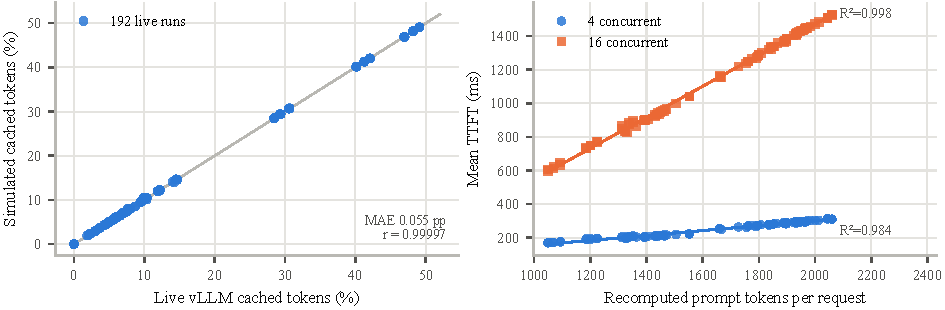
\includegraphics[width=\textwidth]{figures/fidelity.pdf}
\caption{Left: simulated vs.\ live vLLM cached-token fraction for \numfidN{} A100 runs. Right: live mean TTFT is linear in the number of recomputed prompt tokens per request (Qwen2.5-7B-Instruct, 2\,GiB, closed loop).}
\label{fig:fidelity}
\end{figure*}

\section{Pilot Study}
\label{app:pilot}
The pilot used the original synthetic workload: 400 requests from 20 users over HotpotQA, where a fraction (0--75\%) of each request's distractor passages was replaced by passages from a 64-element Zipf-popular pool, together with eight policies (including a design in which the question inherited its evidence scope), three KV budgets, and two concurrency levels, for \numfidN{} runs of vLLM~0.29 with Qwen2.5-7B-Instruct on one A100. It is the source of the fidelity and latency analyses (Figure~\ref{fig:fidelity}), the quality comparison (Table~\ref{tab:quality}), and the overstatement measurement (Section~\ref{sec:synthetic}).

\section{Reproducibility}
\label{app:repro}
All CPU experiments: \texttt{python scripts/run\_v2.py} (about 15 minutes on 10 cores). GPU matrix (4 models $\times$ \{2, 8\} GiB, closed loop, open-loop Poisson rates 4--16\,req/s with a 1\,s TTFT SLO, quality runs with an LLM judge, live insider probe): \texttt{sbatch --array=0-7 scripts/sol\_array.sbatch}, then \texttt{python scripts/analyze\_live\_v2.py} and \texttt{python scripts/make\_paper\_assets.py}, which regenerates every table and number in this paper.

\end{document}
